\section{Bethe Hessian}
\subsection{Principe}
Dans le contexte d'un SBM à 2 communautés 
\subsection{Simulations}
\begin{figure}[H]
	\begin{subfigure}{.5\textwidth}
		\centering
		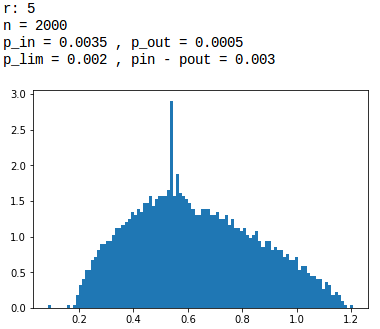
\includegraphics[scale=0.58]{static/bh_5.png}
		\label{bh5}
	\end{subfigure}
	\begin{subfigure}{.5\textwidth}
		\centering
		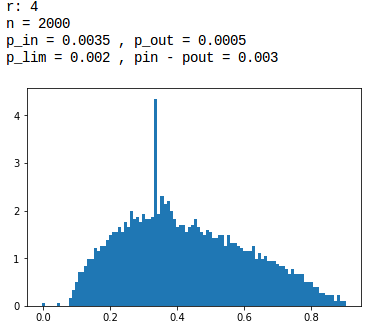
\includegraphics[scale=0.58]{static/bh_3.png}
		\label{bh3}
	\end{subfigure}
	\begin{subfigure}{.5\textwidth}
		\centering
		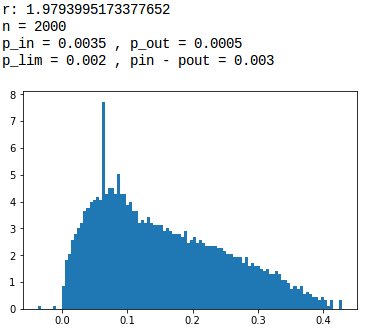
\includegraphics[scale=0.58]{static/bh_2.png}
		\label{bh2}
	\end{subfigure}
	\begin{subfigure}{.5\textwidth}
		\centering
		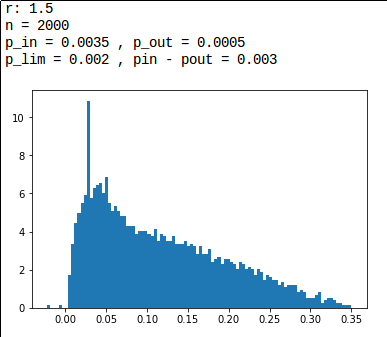
\includegraphics[scale=0.58]{static/bh_1_5.png}
		\label{bh15}
	\end{subfigure}
	\begin{subfigure}{.5\textwidth}
		\centering
		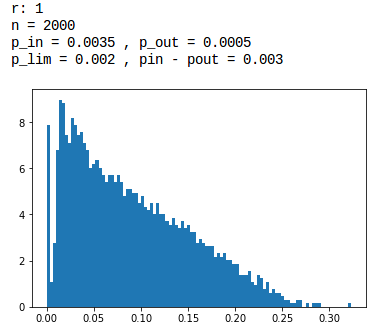
\includegraphics[scale=0.58]{static/bh_1.png}
		\label{bh1}
	\end{subfigure}
	\begin{subfigure}{.5\textwidth}
		\centering
		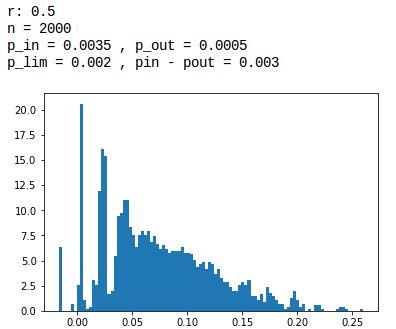
\includegraphics[scale=0.58]{static/bh_0_5.png}
		\label{bh05}
	\end{subfigure}
\end{figure}
\subsection{Theorie}